\documentclass{beamer}
\usepackage[english]{babel}
\usepackage[utf8]{inputenx}
\usepackage{beamerthemeshadow}
\usepackage{Estilos/Estilopres}
\usepackage{color}
\usepackage{listings}
%\usepackage{natbib}
\usepackage{hyperref}
\def\newblock{\hskip .11em plus .33em minus .07em}
\usetheme{Warsaw}
\usecolortheme{dolphin}
\setcounter{tocdepth}{2} %Mostrar solo 3 niveles en el índice
		\makeindex	%índice de palabras
		\title{Other Complexity Classes}
		\subtitle{Computational Complexity}
		\author{\mbox{Luis José Quintana Bolaño}}
		\date{2013-14 Course}


\begin{document}
\frame{\titlepage}

\section{Introduction}
\frame{
\frametitle{Introduction}
    In computational complexity theory, a complexity class is a set of problems of related resource-based complexity. 

    \begin{block}{A typical complexity class has a definition of the form:}The set of problems that can be solved by an abstract machine {\bf M} using {\bf O(f(n))} of resource {\bf R}, where {\bf n} is the size of the input. 
    \end{block}
}
\subsection{Definition}
\frame{
    The simpler complexity classes are defined by the following factors:
    
    \begin {itemize}
    \item {\bf The type of computational problem:} The most commonly used problems are decision problems. However, complexity classes can be defined based on function problems (an example is FP), counting problems (e.g. \#P), optimization problems, promise problems, etc.
    \item {\bf The model of computation:} The most common model of computation is the deterministic Turing machine, but many complexity classes are based on nondeterministic Turing machines, boolean circuits, quantum Turing machines, monotone circuits, etc.
    \item {\bf The resource (or resources) that are being bounded and the bounds:} These two properties are usually stated together, such as "polynomial time", "logarithmic space", "constant depth", etc.
    \end {itemize}

}
\section{Principal Complexity Classes}
\frame{
\frametitle{Time-Bounded Complexity Classes}
    These are some of the most important complexity classes defined by bounding the time of the algorithm:
    \begin{tabular}{|c|c|c|}\hline
    {\bf Class} & {\bf Computational Model} & {\bf Resource Constraint} \\ \hline
    DTIME   &   DTM &   Time $f(n)$ \\ \hline
    P   &   DTM &   Time $poly(n)$  \\ \hline
    EXPTIME &   DTM & Time $2^{poly(n)}$ \\ \hline
    NTIME &	NDTM & Time $f(n)$ \\ \hline
    NP 	& NDTM &	Time $poly(n)$ \\ \hline
    NEXPTIME &	NDTM &	Time $2^{poly(n)}$ \\ \hline   
    \end{tabular}

}
\frame{
\frametitle{Space-Bounded Complexity Classes}
    Some examples of classes defined by bounding the space of the algorithm:
    \begin{tabular}{|c|c|c|}\hline
    {\bf Class} & {\bf Computational Model} & {\bf Resource Constraint} \\ \hline
    DSPACE & 	DTM &	Space $f(n)$ \\ \hline
    L 	& DTM &	Space $O(\log n)$ \\ \hline
    L$^2$ & DTM & Space $O(\log^2 n)$ \\ \hline
    PSPACE &	DTM &	Space $poly(n)$ \\ \hline
    EXPSPACE &	DTM &	Space $2^{poly(n)}$ \\ \hline
    NSPACE & 	NDTM &	Space $f(n)$ \\ \hline
    NL &	NDTM & Space $O(\log n)$ \\ \hline
    NPSPACE &	NDTM &	Space $poly(n)$ \\ \hline
    NEXPSPACE &	NDTM &	Space $2^{poly(n)}$ \\ \hline
    \end{tabular}
}
\frame{
\frametitle{Relations Between Time- and Space-Bounded Classes}
    \begin{figure}[!h]
  			\centering
  			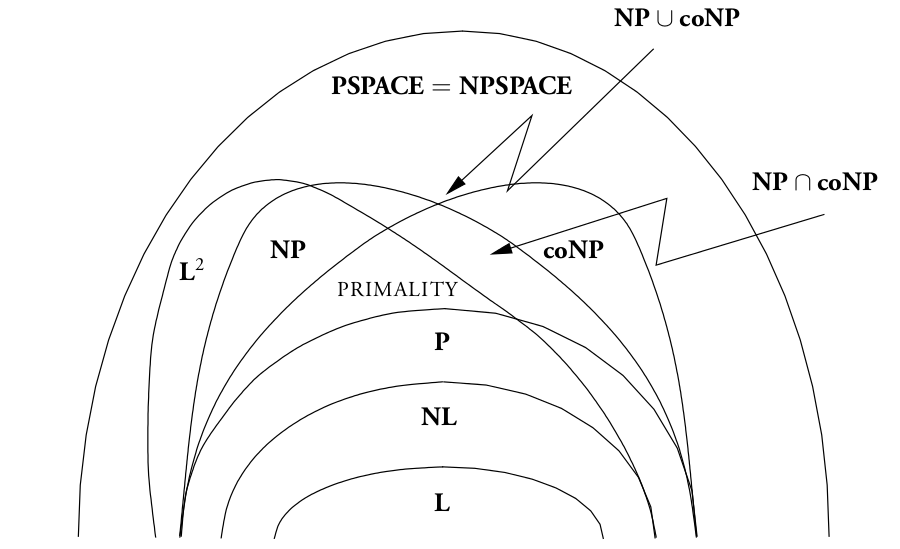
\includegraphics[width=0.60\textwidth,clip]{relations.png}
  			\caption{The relationships among complexity classes}
  	\end{figure}
    \begin{block}{}
    \begin{center}
    $\mbox{L} \subseteq \mbox{NL} \subseteq \mbox{P} \subseteq \mbox{NP} \subseteq \mbox{PSPACE} \subseteq \mbox{EXPTIME} \subseteq \mbox{NEXPTIME}$ \\ Where \\
     $\mbox{PSPACE} = \mbox{NPSPACE}$ and $\mbox{P} \subset \mbox{EXPTIME}$
    \end{center}\end{block}
}
\frame{
\frametitle{Other classes}
    Other important complexity classes that use different computational models include:
    \begin{itemize}
    \item BPP, ZPP and RP, which are defined using probabilistic Turing machines.
    \item AC and NC, which are defined using boolean circuits.
    \item BQP and QMA, which are defined using quantum Turing machines.
    \end{itemize}
}
\frame{
\section{Complementary Classes}
\frametitle{Complementary Classes}
    Complexity classes have a variety of closure properties; for example, decision classes may be closed under negation, disjunction, conjunction, or even under all Boolean operations.
    \begin{block}{Definition}
    Each {\bf class X} that is {\bf not closed under negation} has a {\bf complement class co-Y}, which consists of the complements of the languages contained in X.
    \end{block} 
}
\frame{
    \begin{exampleblock}{Example}
    For the {\bf NP} class there's a {\bf coNP} class which, for every decision problem {\it P} in {\bf NP}, contains the complementary decision problem, denoted {\it coP} (i.e., the decision problem in which the “Yes” instances are “No” instances of {\bf P} and vice versa).
    \end{exampleblock}
    \begin{block}{}If {\bf C} is a deterministic time or space complexity class, then {\bf coC} = {\bf C}.\end{block}
}
\frame{
\section{References}
\frametitle{References}
    \nocite{*}
    \bibliographystyle{alpha}
    \bibliography{biblio.bib}
}
\end{document}
